\documentclass{memoria}
\usepackage{algorithm}
\usepackage{algpseudocode}
\usepackage{float}
\usepackage{multirow}
\usepackage{graphicx}
\usepackage{subcaption}
\usepackage{hyperref}
\usepackage{adjustbox}
\setcounter{secnumdepth}{4}
\usepackage[table,xcdraw]{xcolor}

\algdef{SE}[VARIABLES]{Variables}{EndVariables}
   {\algorithmicvariables}
   {\algorithmicend\ \algorithmicvariables}
\algnewcommand{\algorithmicvariables}{\textbf{global variables}}

\begin{document}
\pagestyle{empty} % retira numeracion de paginas
%datos%
\author{Luis González Romero, XXXXXXXXX, luisgonromero@correo.ugr.es}
\title{Práctica 2: Visualización y Segmentación}
\newcommand{\grupopracticas}{Grupo 1: Miércoles 17:30-19:30}
\newcommand{\subtitulo}{Subtítulo}
\newcommand{\curso}{Inteligencia de Negocio}
\newcommand{\departamento}{Computación y Sistemas Inteligentes}

\begin{center}
\LARGE{\bf \thetitle:}\\
%\Large{\bf \subtitulo}\\
\end{center}

%\vspace{1em}


%\vfill


\begin{figure}[H]
\centering

\includegraphics[scale=0.8]{imagenes/logo.png}
\end{figure}


\begin{center}
\theauthor
\\
%\grupopracticas
\end{center}

\begin{center}
Escuela Técnica Superior de Ingeniería informática y Telecomunicaciones

\end{center}

%\vspace{2in}

\begin{center}
\today
%\displaydate{date}
\end{center}
%\afterpage{\blankpage \addtocounter{page}{1}} %addtocounter incrementa numero de pagina ya que blankpage no lo hace%

\newpage
\begin{center}
%\theauthor
\end{center}
\vspace{3in}
\begin{center}
\LARGE{\thetitle}\\
\end{center}

\vspace{2in}

\begin{flushright}
Memoria sobre la tercera práctica de la asignatura \curso \\ cursada en la ETSIIT, UGR.
\\
\vspace{0.2in}

\theauthor


\end{flushright}

\vfill
\begin{center}
%\today
\end{center}

\newpage

\pagestyle{plain} %muestra numeracion de paginas%
\tableofcontents

%Lista de figuras%
%\renewcommand{\listfigurename}{\centering LISTA DE FIGURAS}
\listoffigures
%\newpage

%Lista de tabelas%
%\renewcommand{\listtablename}{\centering Índice de tablas}
\listoftables
%\newpage

%Sumario%

\newpage
\section{Leaderboard}

En Kaggle me di de alta como LuisUGR, ya que en la primera clase en la que se explicó el guión se dijo que usaramos: -DNI o -UGR. Dias después, intenté cambiarlo pero siempre salía que se había cambiado con éxito, pero realmente no se aplicaba.

\begin{figure}[H]
\centering
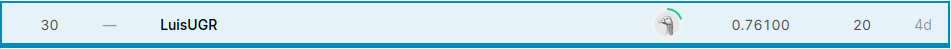
\includegraphics[width=\textwidth]{imagenes/leaderboard.png}
\caption{Fila de la competición correspondiente}
\end{figure}

\section{Predicción de precios de coches usados}

\subsection{Descripción del problema}

Tenemos un conjunto de datos de vehículos usados, clasificados estos en 5 categorías: del 1 al 5 dependiendo del precio(desde los más baratos a más caros, respectivamente). Debemos de poder predecir la categoría a la que pertenece un coche(clasificación multiclase).

\begin{figure}[H]

\begin{subfigure}{.5\textwidth}
  \centering
  \includegraphics[width=0.8\textwidth]{imagenes/features/Año.png}
  \caption{Año}
\end{subfigure}%
\begin{subfigure}{.5\textwidth}
  \centering
  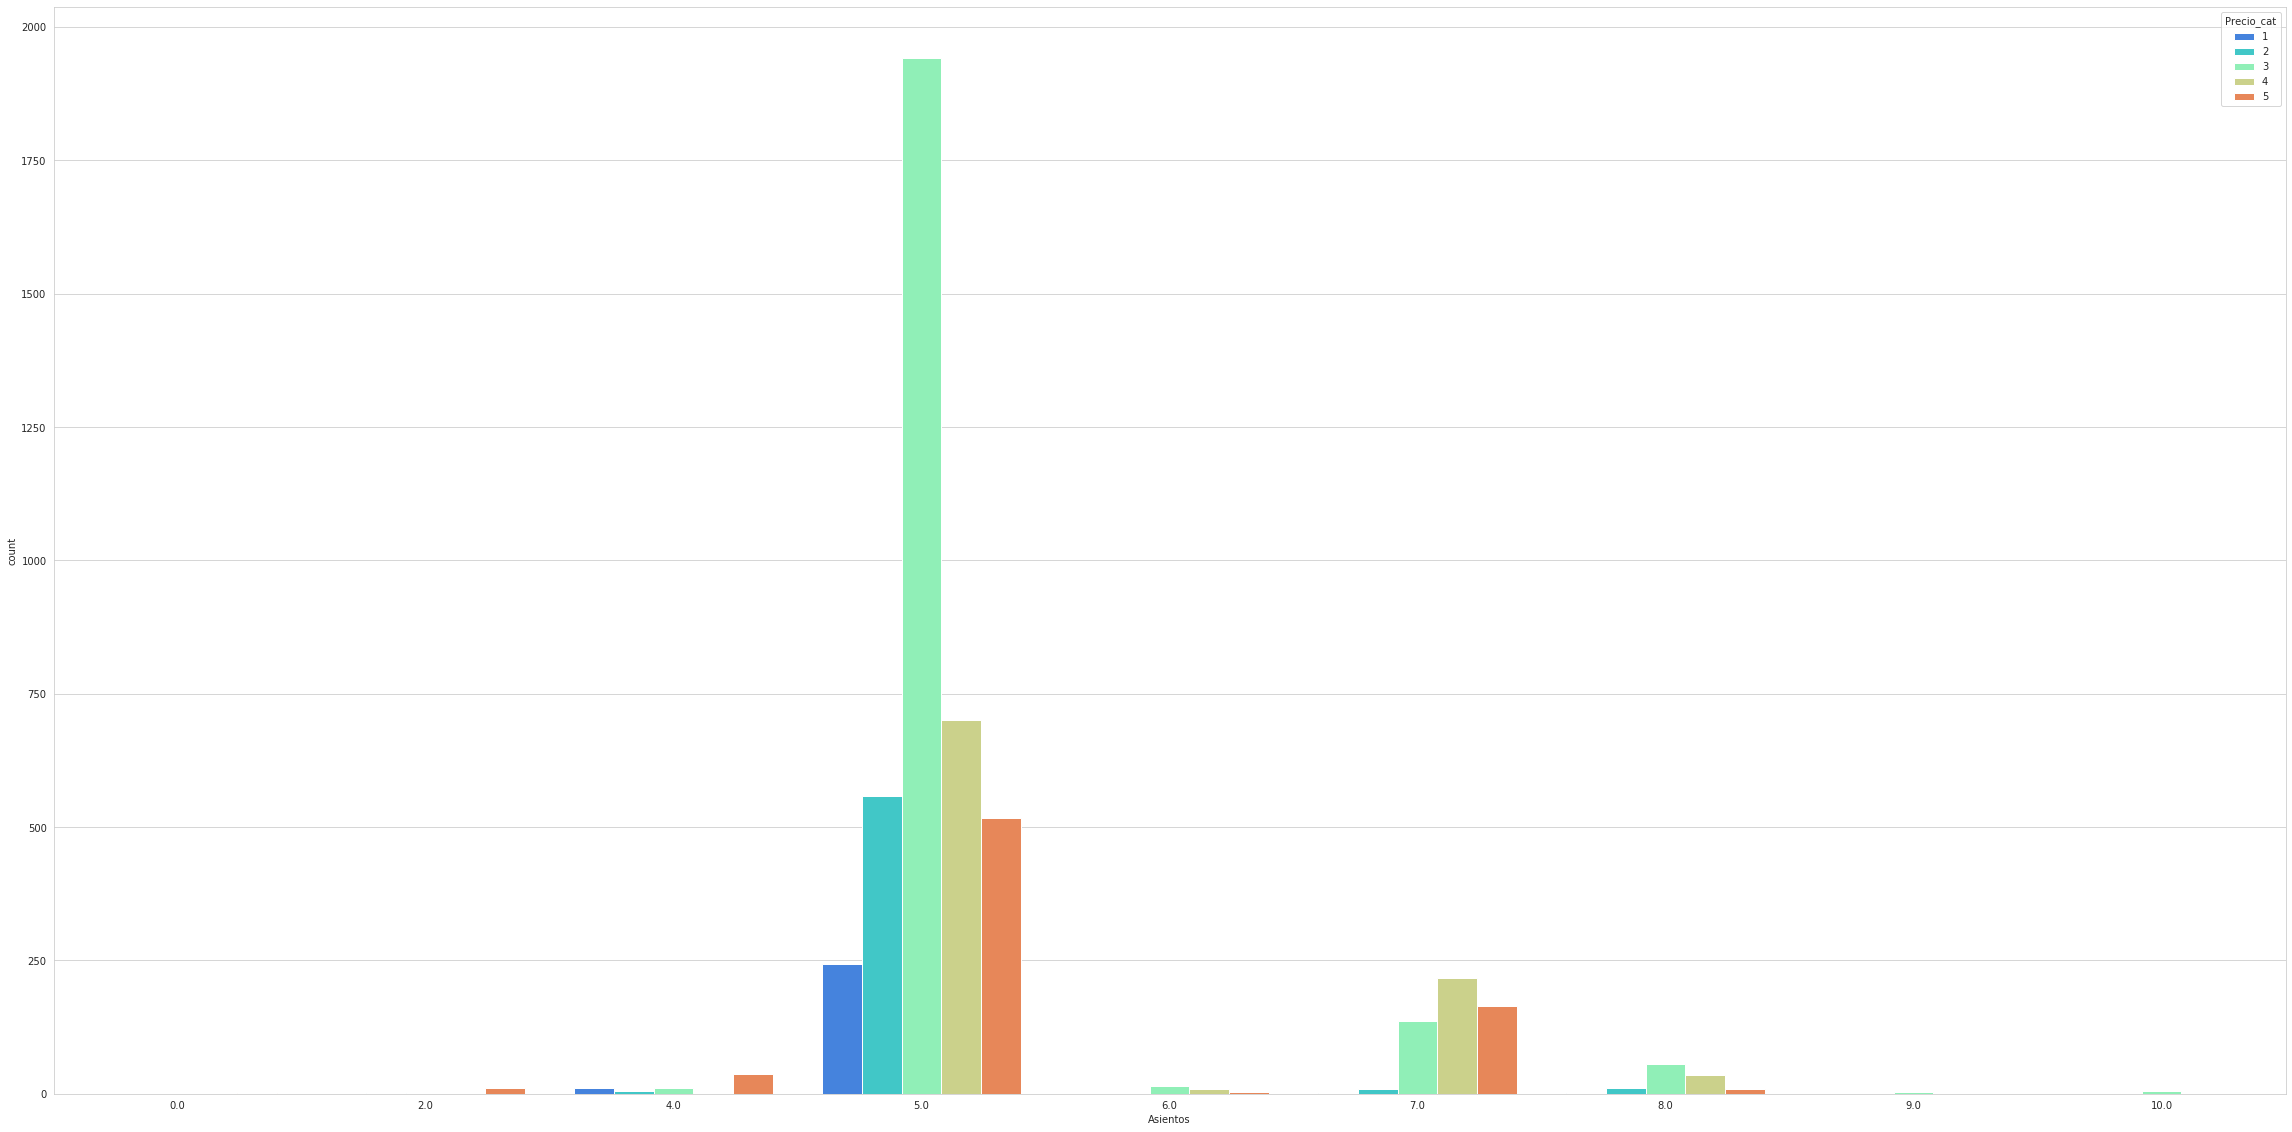
\includegraphics[width=0.8\textwidth]{imagenes/features/Asientos.png}
  \caption{Asientos}
\end{subfigure}
\begin{subfigure}{.5\textwidth}
  \centering
  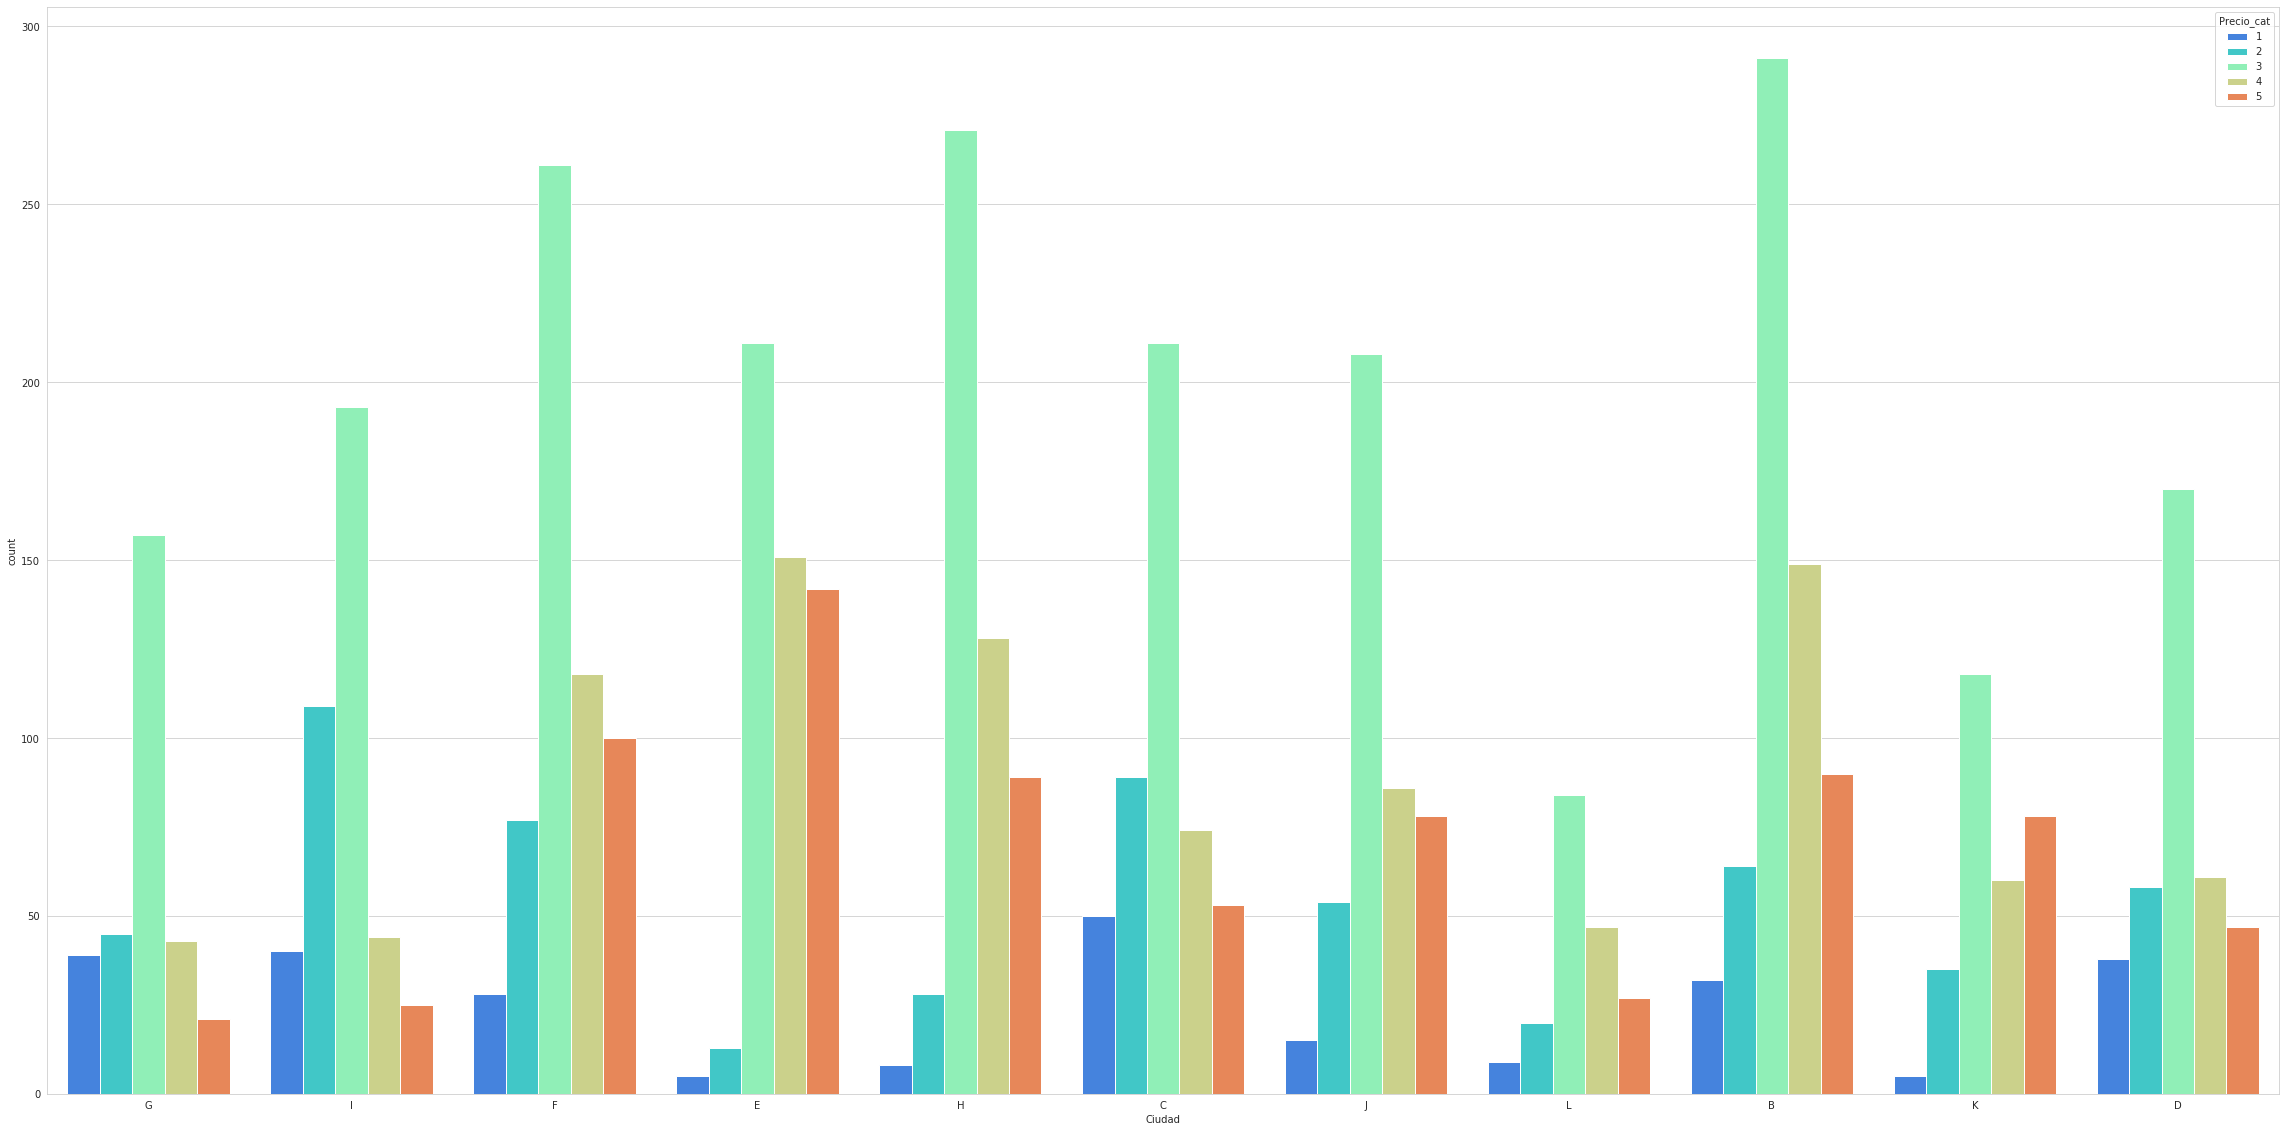
\includegraphics[width=0.8\textwidth]{imagenes/features/Ciudad.png}
  \caption{Ciudad}
\end{subfigure}%
\begin{subfigure}{.5\textwidth}
  \centering
  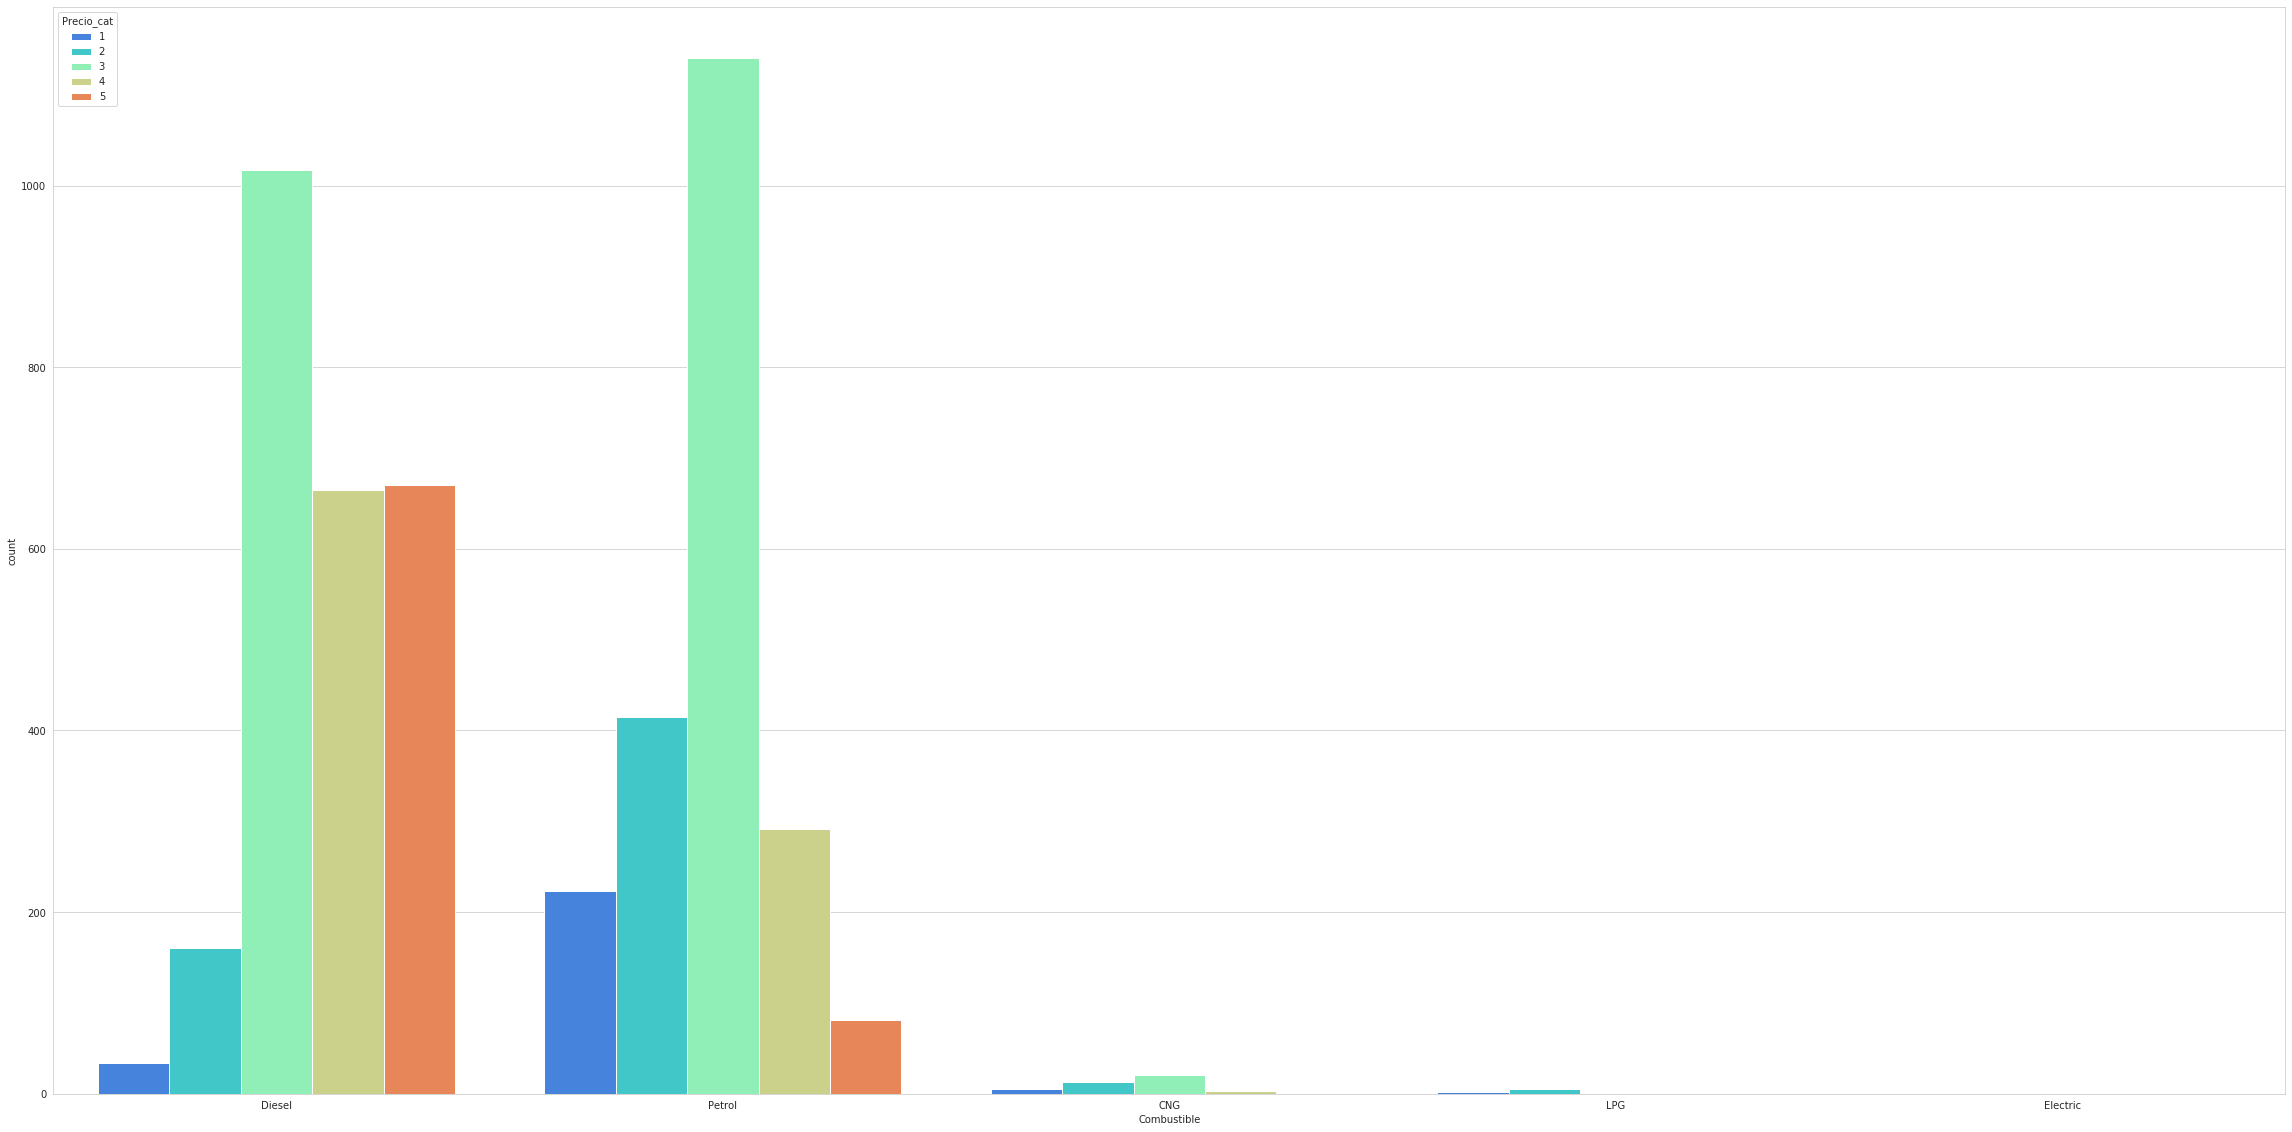
\includegraphics[width=0.8\textwidth]{imagenes/features/Combustible.png}
  \caption{Combustible}
\end{subfigure}
\begin{subfigure}{.5\textwidth}
  \centering
  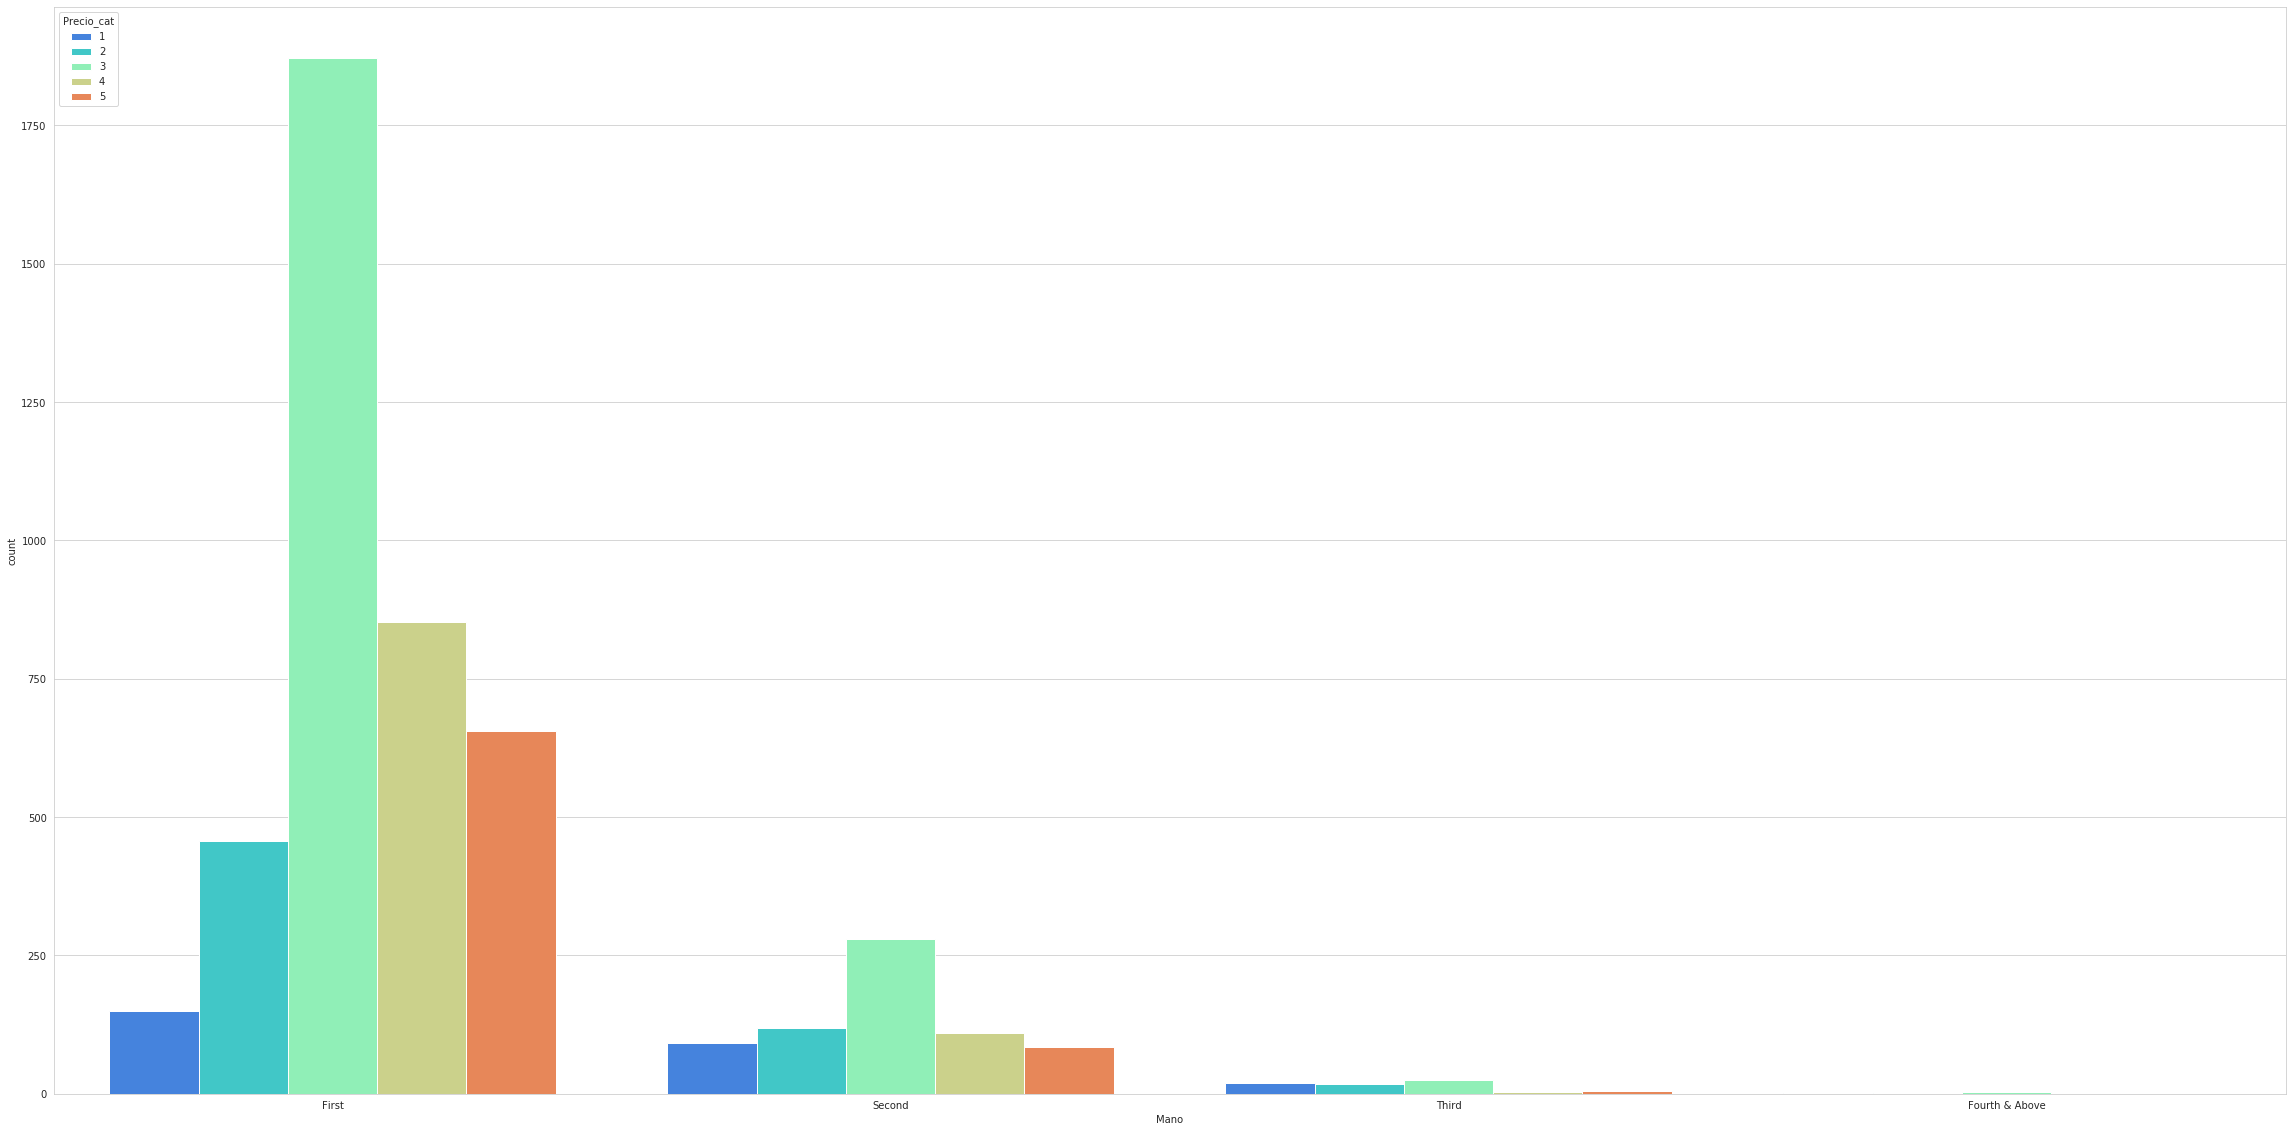
\includegraphics[width=0.8\textwidth]{imagenes/features/Mano.png}
  \caption{Mano}
\end{subfigure}%
\begin{subfigure}{.5\textwidth}
  \centering
  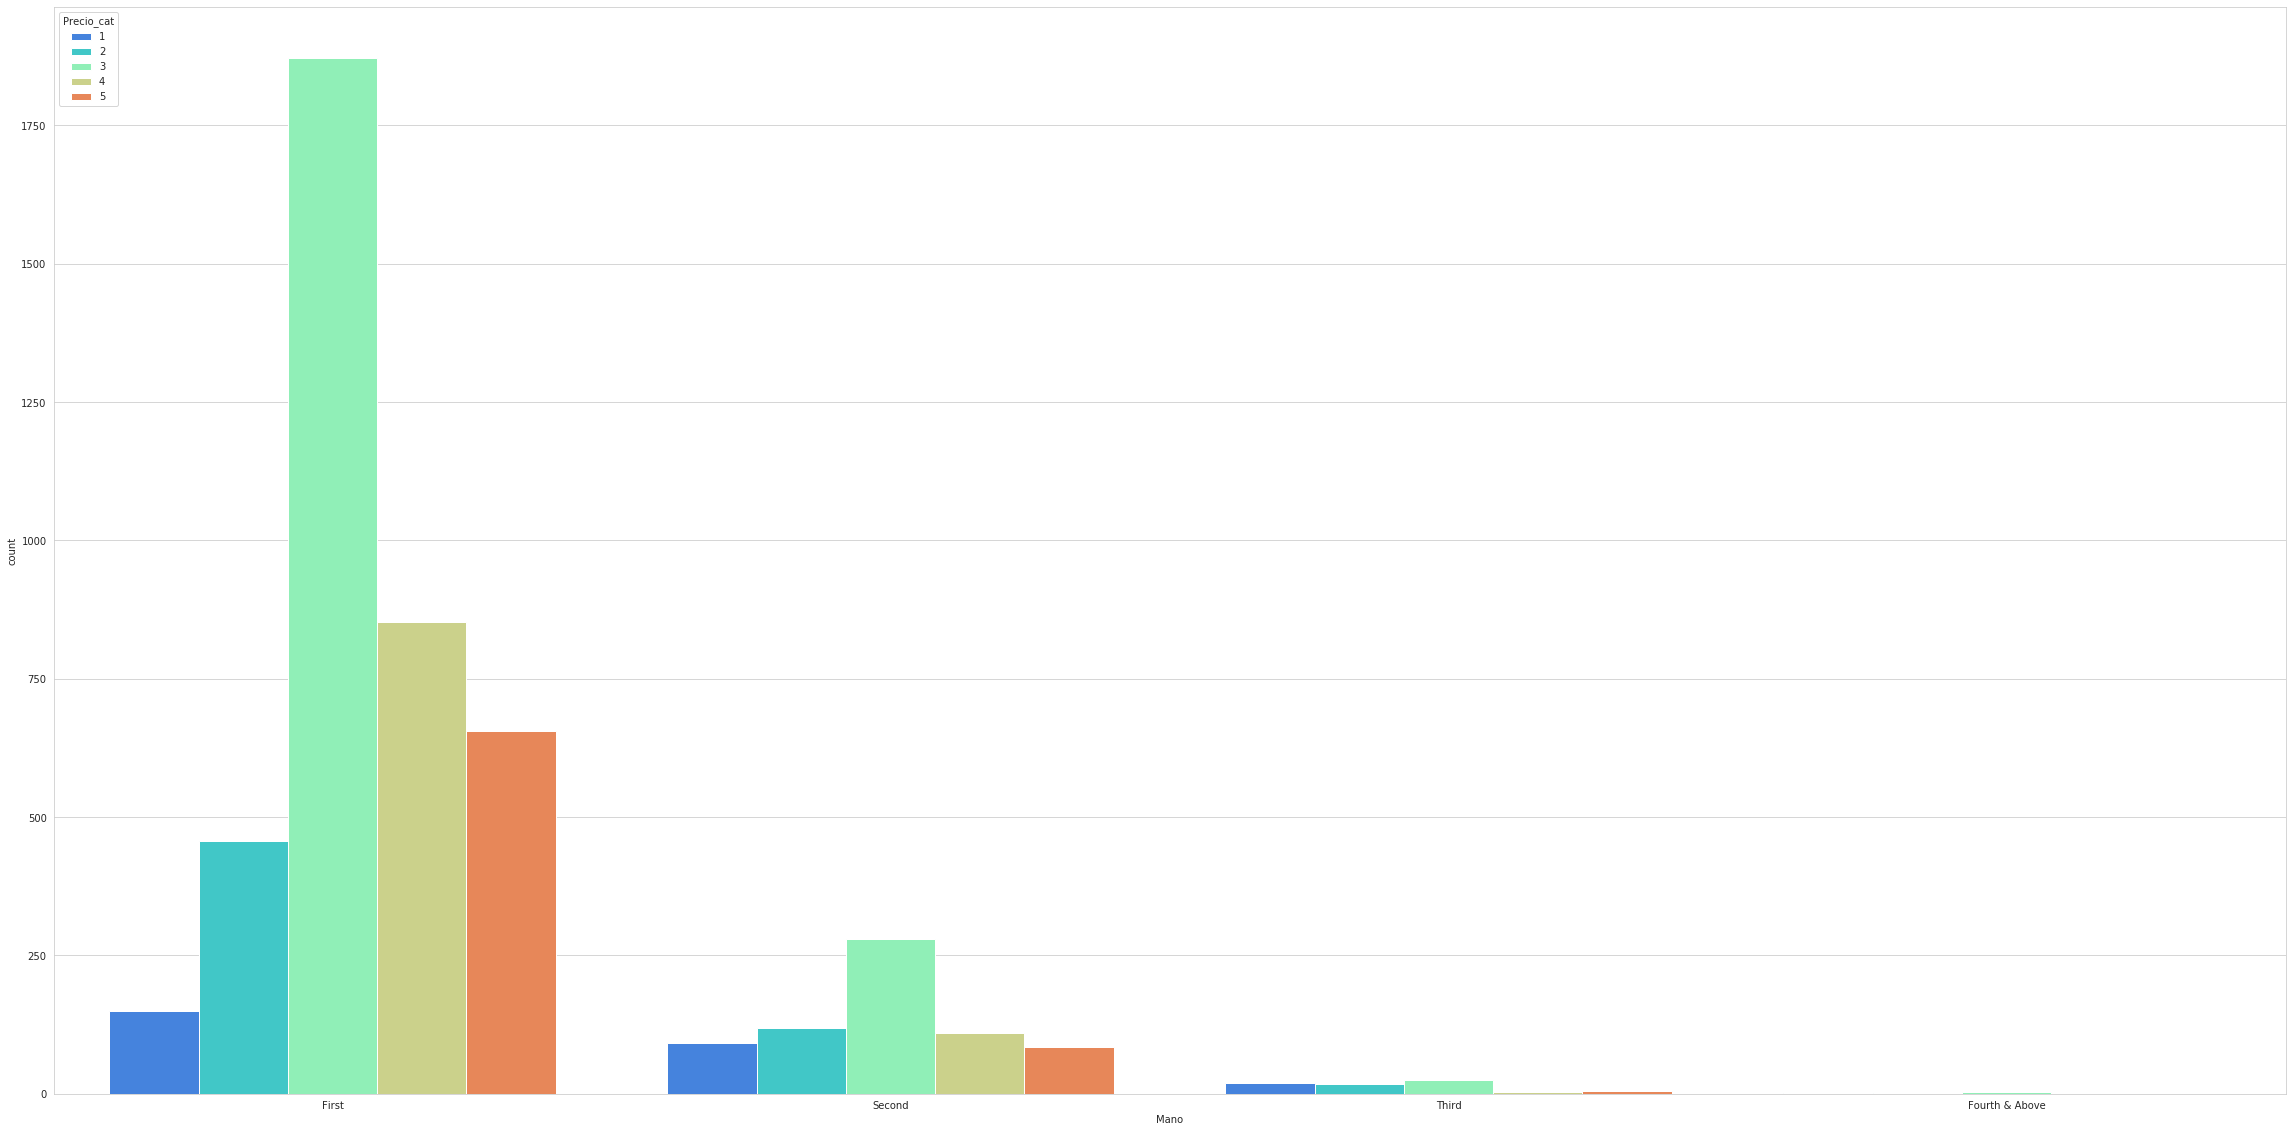
\includegraphics[width=0.8\textwidth]{imagenes/features/Mano.png}
  \caption{Mano}
\end{subfigure}
\begin{subfigure}{.5\textwidth}
  \centering
  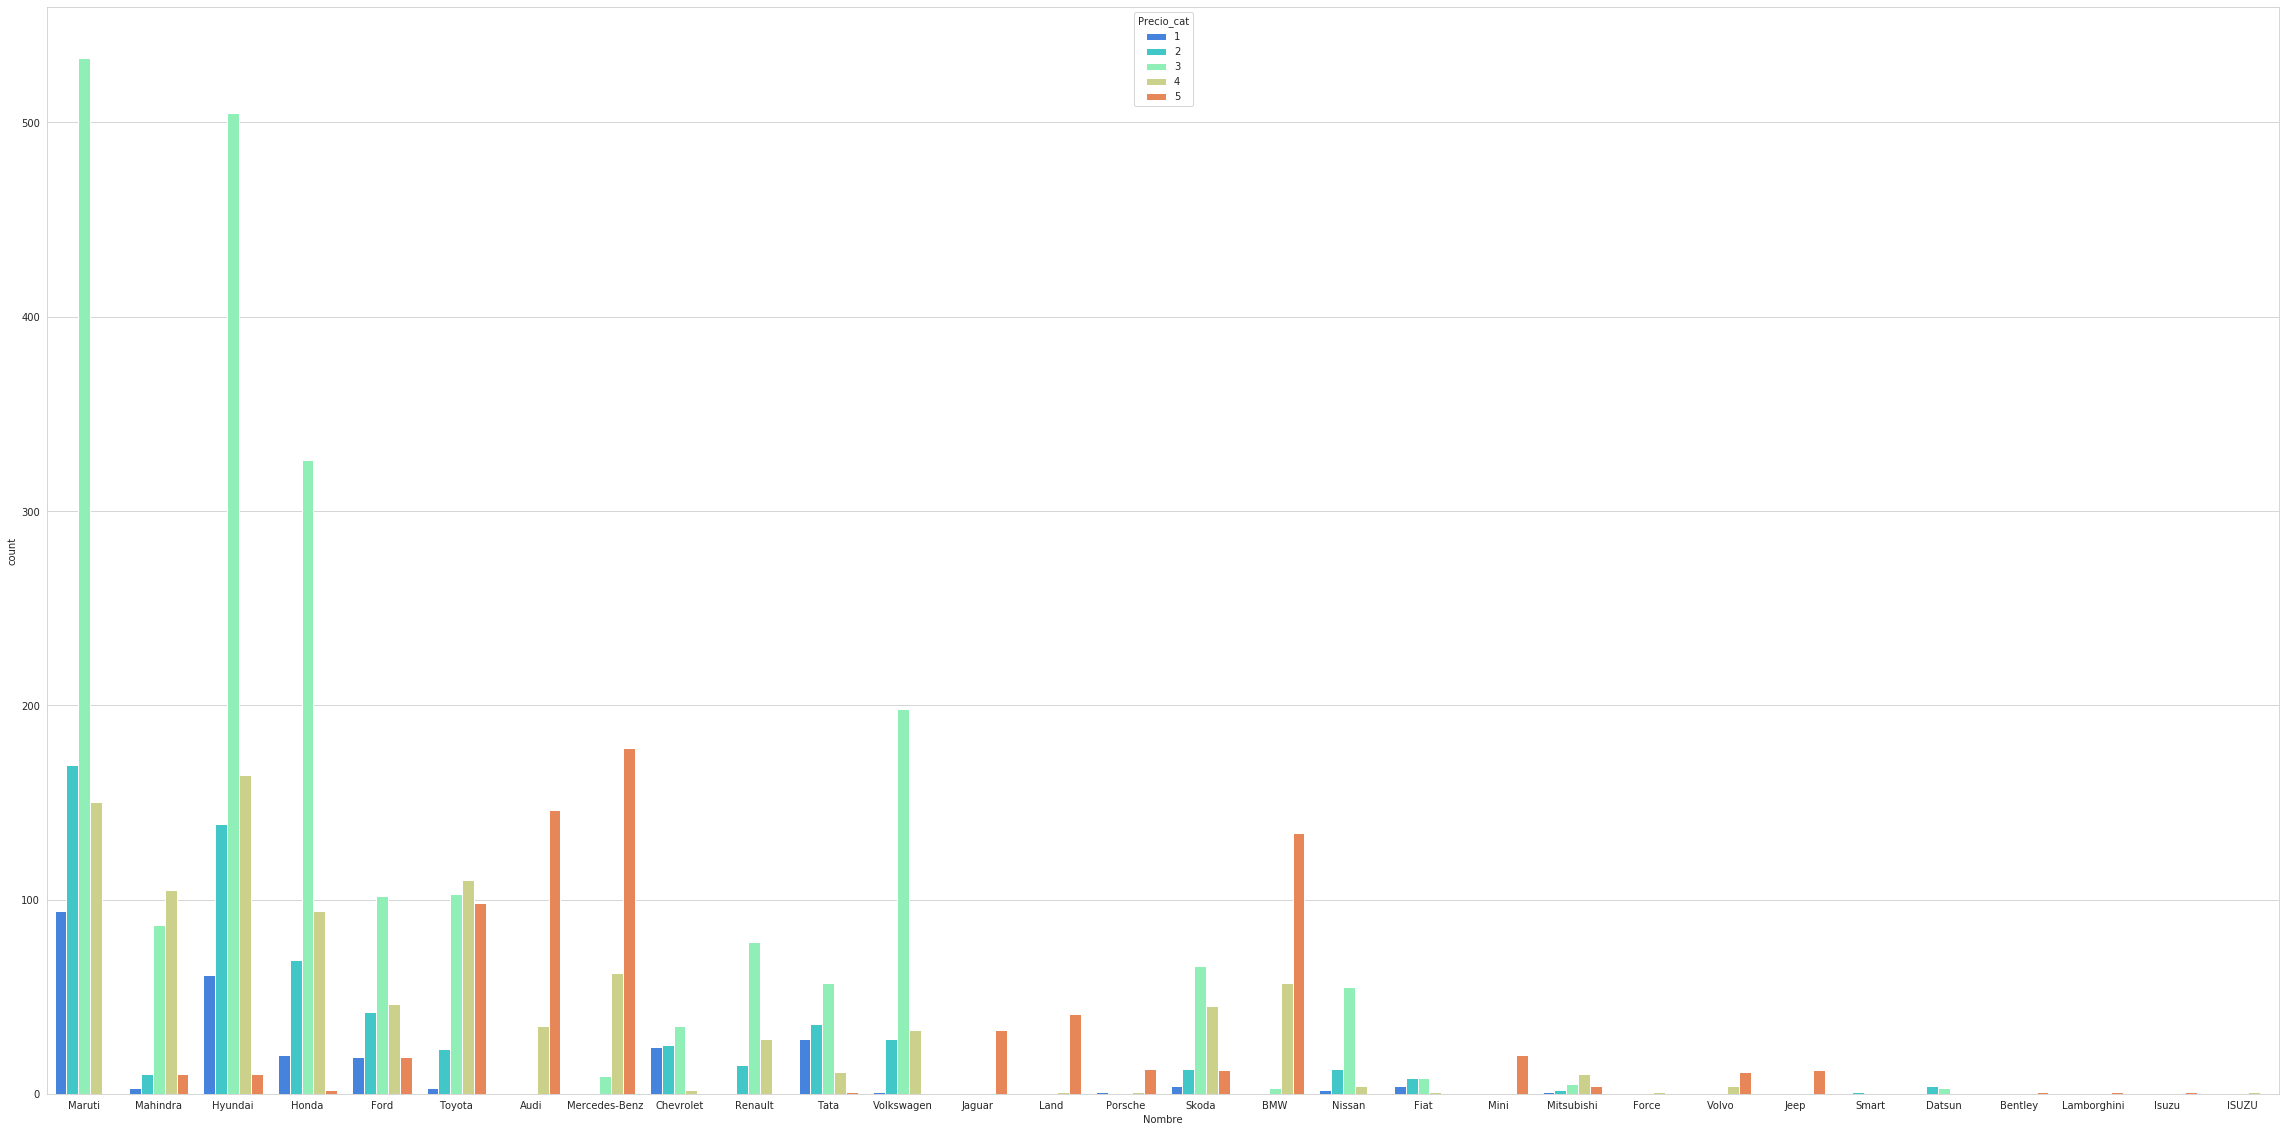
\includegraphics[width=0.8\textwidth]{imagenes/features/Nombre.png}
  \caption{Marca del vehículo}
\end{subfigure}%
\begin{subfigure}{.5\textwidth}
  \centering
  \includegraphics[width=0.8\textwidth]{imagenes/features/Tipo_Marchas.png}
  \caption{Tipo de marchas}
\end{subfigure}

\caption{Presencia de cada variable en las distintas clases representadas en Precio\_cat}
\label{fig:fig}
\end{figure}

\begin{figure}[H]
\centering
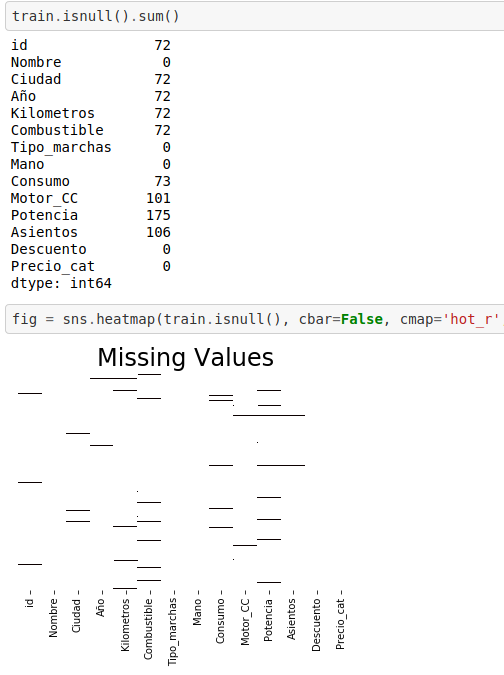
\includegraphics[width=0.8\textwidth]{imagenes/mv.png}
\caption{Valores perdidos en el dataset de entrenamiento.}
\end{figure}

\begin{figure}[H]
\centering
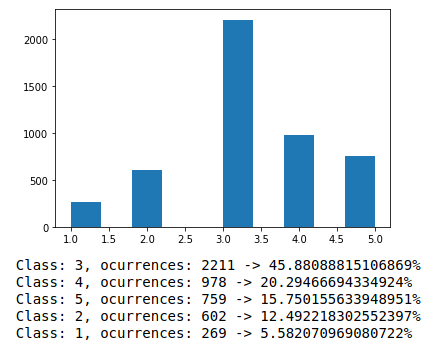
\includegraphics[width=0.8\textwidth]{imagenes/classes.png}
\caption{Ocurrencias de las clases}
\end{figure}

Como bien sabíamos, se trata de un problema con múltiples clases y en este caso, desbalanceadas.

\section{Subidas a la plataforma Kaggle}

\subsection{Resumen de las subidas}

Las subidas 13 y 19 no aparecen porque subí un csv donde la columna de etiquetas tenía formato erróneo(equivalentes a las posteriores a estas), por lo que obtuve score $0,00$.

\begin{table}[H]
\centering
\begin{tabular}{|c|c|c|c|c|}
\hline
\textbf{Submission} & \textbf{Date} & \textbf{Private Score}         & \textbf{Local Score} & \textbf{Description} \\ \hline
\textit{1}          & 17-12         & {\color[HTML]{134F5C} 0,73943} & 0,801064             &      $prep_{sin\_mv}$, \textit{rfc} y $features_{1}$             \\ \hline
\textit{2}          & 17-12         & {\color[HTML]{134F5C} 0,72562} & 0,885873             &         $prep_{sin\_mv}$, \textit{rfc}, $features_{1}$                        y $over_{1}$ \\ \hline
\textit{3}          & 17-12         & {\color[HTML]{134F5C} 0,72562} & 0,805373             &       $prep_{sin\_mv}$, \textit{xgb} y $features_{1}$                           \\ \hline
\textit{4}          & 18-12         & {\color[HTML]{134F5C} 0,74547} & 0,901131             &        $prep_{2}$, \textit{xgb}, $features_{1}$ y $over_{1}$                                        \\ \hline
\textit{5}          & 19-12         & {\color[HTML]{134F5C} 0,75496} & 0,889281            &        $prep_{2}$, \textit{xgb-tuning}, $features_{1}$ y $over_{1}$               \\ \hline
\textit{6}          & 22-12         & {\color[HTML]{134F5C} 0,75754} & 0,800581             &        $prep_{2}$, \textit{lgb}, $features_{1}$              \\ \hline
\textit{7}          & 22-12         & {\color[HTML]{134F5C} 0,64106} & 0,948383             &            $prep_{2}$, \textit{lgb}, $features_{1}$,                       $over_{1}$, $under_{1}$ \\ \hline
\textit{8}          & 22-12         & {\color[HTML]{00F000} 0,76100}    & 0,970485             &        $prep_{2}$, \textit{lgb}, $features_{1}$, $over_{3}$                            \\ \hline
\textit{9}          & 23-12         & {\color[HTML]{F00000} 0,62381}    & 0,907092             &        $prep_{2}$, \textit{lgb}, $features_{1}$, $over_{4}$              \\ \hline
\textit{10}         & 23-12         & {\color[HTML]{134F5C} 0,72303} & 0,800374             &       $prep_{2}$, \textit{rfc-gridsearch}, $features_{1}$               \\ \hline
\textit{11}         & 24-12         & {\color[HTML]{134F5C} 0,73856} & 0,761826             &       $prep_{2}$, \textit{stacking}, $features_{1}$               \\ \hline
\textit{12}         & 24-12         & {\color[HTML]{134F5C} 0,73770} & 0,712209             &      $prep_{2}$, \textit{stacking}, $features_{1}$, $under_{2}$                \\ \hline
\textit{14}         & 25-12         & {\color[HTML]{134F5C} 0,72389} & -             &             $prep_{2}$, \textit{catboost}, $features_{1}$                        \\ \hline
\textit{15}         & 25-12         & {\color[HTML]{134F5C} 0,72821} & 0,840249             &           $prep_{2}$, \textit{catboost}, $features_{1}$                          \\ \hline
\textit{16}         & 27-12         & {\color[HTML]{134F5C} 0,73425} & 0,747925             &       $prep_{2}$, \textit{lgb-tuning}, $smote+tomek\_ links$               \\ \hline
\textit{17}         & 27-12         & {\color[HTML]{134F5C} 0,71613} & 0,718880             &         $prep_{2}$, \textit{lgb}, $smote+tomek\_ links$ \\ \hline
\textit{18}         & 27-12         & {\color[HTML]{134F5C} 0,73684} & 0,786492             &      $prep_{2}$, \textit{lgb}, $smote+tomek\_ links$                \\ \hline
\textit{20}         & 31-12         & {\color[HTML]{134F5C} 0,75323} & 0,738589             &           $prep_{knn}$, \textit{lgb}, $features_{2}$          \\ \hline
\end{tabular}
\caption{Subidas a la plataforma Kaggle}
\end{table}

\begin{figure}[H]
\centering
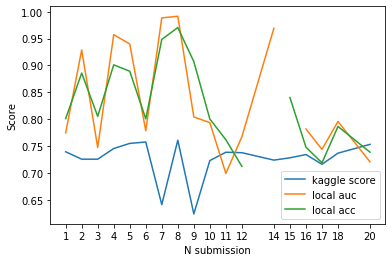
\includegraphics[width=0.6\textwidth]{imagenes/subs-graph.png}
\caption{Representación gráfica de los score obtenidos en Kaggle.}
\end{figure}

\begin{table}[H]
\centering
\begin{tabular}{|c|c|c|c|}
\hline
\textbf{Submission} & \textbf{Private Score}         & \textbf{Local AUC} & \textbf{Local Acc} \\ \hline
\textit{1}          & {\color[HTML]{134F5C} 0,73943} & 0,774507           & 0,801064           \\ \hline
\textit{2}          & {\color[HTML]{134F5C} 0,72562} & 0,928768           & 0,885873           \\ \hline
\textit{3}          & {\color[HTML]{134F5C} 0,72562} & 0,747393           & 0,805373           \\ \hline
\textit{4}          & {\color[HTML]{134F5C} 0,74547} & 0,957258           & 0,901131           \\ \hline
\textit{5}          & {\color[HTML]{134F5C} 0,75496} & 0,939908           & 0,889281           \\ \hline
\textit{6}          & {\color[HTML]{134F5C} 0,75754} & 0,778514           & 0,800581           \\ \hline
\textit{7}          & {\color[HTML]{134F5C} 0,64106} & 0,988479           & 0,948383           \\ \hline
\textit{8}          & {\color[HTML]{00F000} 0,76100}    & 0,991525           & 0,970485           \\ \hline
\textit{9}          & {\color[HTML]{F00000} 0,62381}    & 0,804244           & 0,907092           \\ \hline
\textit{10}         & {\color[HTML]{134F5C} 0,72303} & 0,793589           & 0,800374           \\ \hline
\textit{11}         & {\color[HTML]{134F5C} 0,73856} & 0,699132           & 0,761826           \\ \hline
\textit{12}         & {\color[HTML]{134F5C} 0,73770} & 0,767308           & 0,712209           \\ \hline
\textit{14}         & {\color[HTML]{134F5C} 0,72389} & 0,969275           & -                  \\ \hline
\textit{15}         & {\color[HTML]{134F5C} 0,72821} & -                  & 0,840249           \\ \hline
\textit{16}         & {\color[HTML]{134F5C} 0,73425} & 0,781858           & 0,747925           \\ \hline
\textit{17}         & {\color[HTML]{134F5C} 0,71613} & 0,743823           & 0,718880           \\ \hline
\textit{18}         & {\color[HTML]{134F5C} 0,73684} & 0,795716           & 0,786492           \\ \hline
\textit{20}         & {\color[HTML]{134F5C} 0,75323} & 0,720588           & 0,738589           \\ \hline
\end{tabular}
\caption{Subidas con dos medidas}
\end{table}

\subsection{Selección de columnas}

\begin{figure}[H]

\begin{subfigure}{.5\textwidth}
  \centering
  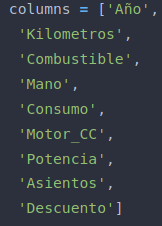
\includegraphics[width=0.5\textwidth]{imagenes/cols1.png}
  \caption{$features_{1}$}
  \label{fig:sfig1}
\end{subfigure}%
\begin{subfigure}{.5\textwidth}
  \centering
  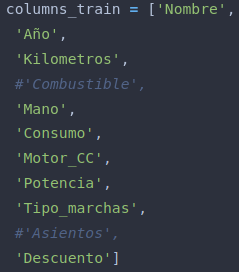
\includegraphics[width=0.5\textwidth]{imagenes/cols2.png}
  \caption{$features_{2}$}
  \label{fig:sfig2}
\end{subfigure}

Se transformaron las columnas \textit{Consumo}, \textit{Motor\_CC} y \textit{Potencia} de cadena a \textit{real}, haciendo uso de expresiones regulares.

\begin{figure}[H]
\centering
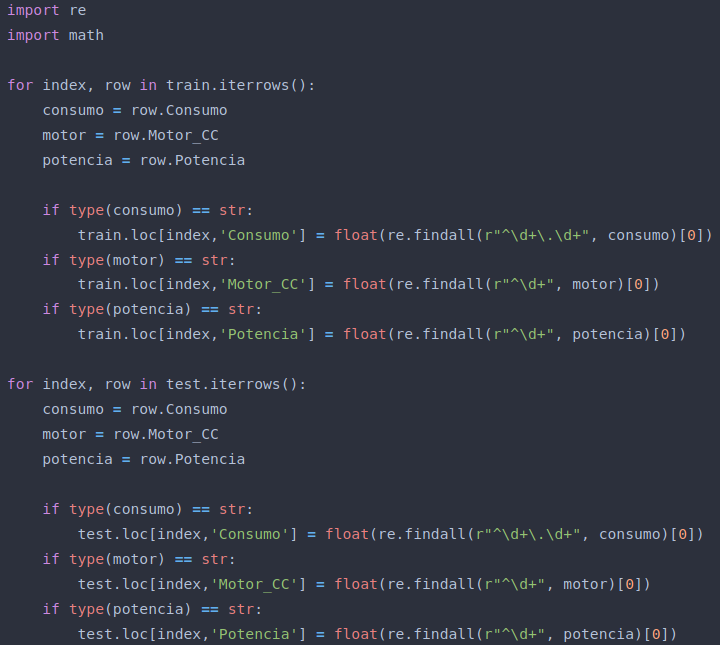
\includegraphics[width=0.6\textwidth]{imagenes/er.png}
\caption{Obteniendo el valor de las columnas \textit{Consumo}, \textit{Motor\_CC} y \textit{Potencia}}
\end{figure}

\caption{Selección de columnas usado}
\label{fig:fig}
\end{figure}

\subsection{Imputación de valores perdidos}

\begin{itemize}

\item $prep_{sin\_mv} \rightarrow$ data\_without\_nan = train.copy()
\newline	
	data\_without\_nan = data\_without\_nan.dropna()
	
\item $prep_{2}$ $\rightarrow $ Imputación de valores nulos: categóricos-most\_freq y numéricos-mean

\item $prep_{knn} \rightarrow  KNNImputer(n\_neighbors=5, weights='uniform', metric='nan\_euclidean')$

\end{itemize}

\subsection{Oversamplers}

Para los $smote\_variants$, he usado \textit{MulticlassOversampling}, pasándole la variante que especifico como parámetro(oversampler=variante).

\begin{itemize}
\item $over_{1} \rightarrow imblearn.over\_sampling.SMOTE$
\item $over_{2} \rightarrow smote\_variants.MDO$
\item $over_{3} \rightarrow smote\_variants.DSRBF$
\item $over_{4} \rightarrow smote\_variants.MSMOTE$
\end{itemize}

\subsection{Undersamplers}
\begin{itemize}
\item $under_{1} \rightarrow smote\_variants.EditedNearestNeighbors()$
\item $under_{2} \rightarrow smote\_variants.CondensedNearestNeighbour()$
\item $under_{3} \rightarrow $ \textit{Tomek links}
\end{itemize}

\subsection{subida 1}
La primera subida consite en usar Random Forest como clasificador, pasándole como parámetro la semilla que esta en todos los notebooks igual.

Para la validación cruzada se usará:
$cv\_ = StratifiedKFold(n\_splits=5, shuffle=True)$

$rfc = RandomForestClassifier(random\_state=random\_seed)$\newline
$y\_pred = cross\_val\_predict(rfc, X, y, cv=cv\_, n\_jobs=-1)$

\subsection{subida 2}

Igual que la anterior pero haciendo oversampling.

$from$ $imblearn.over\_sampling$ $import$ $SMOTE$\newline
$oversample = SMOTE()$\newline
$X, y = oversample.fit\_resample(X, y)$\newline

\subsection{subida 3}

Igual que la primera pero usando \textit{XGBClassifier} con parámetros por defecto.

\subsection{subida 4}

Igual que la anterior pero haciendo $prep_{2}$ y $SMOTE_{imblearn}$.

\subsection{subida 5}

% mirar si cambiar SMOTE por SMOTE_{imblearn}
Igual que el anterior pero haciendo tuning de parámetros.

\begin{figure}[H]
\centering
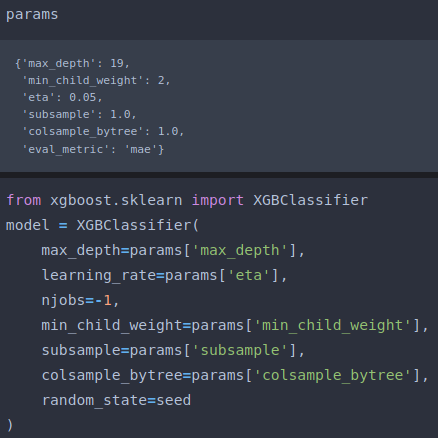
\includegraphics[width=0.8\textwidth]{imagenes/sub5.png}
\caption{Hyperparameter tuning(XGB) - sub5}
\end{figure}

\subsection{subida 6}

Igual que sub3 pero usando \textit{lgb} como clasificador.

$clf = lgb.LGBMClassifier(random\_state=seed, n\_jobs=-1)$

\subsection{subida 7}

Igual que la anterior pero haciendo uso de $over_{2}$ y $under_{1}$.

\subsection{subida 8}

Igual que sub6 pero haciendo uso de $over_{3}$.

\subsection{subida 9}

Igual que la anterior pero empleando $over_{4}$.

\subsection{subida 10}

A partir de esta subida, realizo una estandarización de los datos de entrenamiento y test.

\begin{figure}[H]
\centering
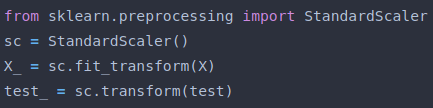
\includegraphics[width=0.4\textwidth]{imagenes/sub10-norm.png}
\caption{\textit{sklearn.preprocessing.StandardScaler}}
\end{figure}

Para esta subida hice un ranking previo de clasificadores para escoger uno al que realizar un \textit{GridSearchCV}, en este caso mirando F1-score.

\begin{figure}[H]
\centering
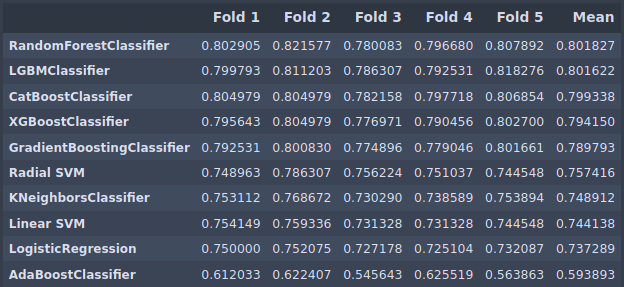
\includegraphics[width=0.8\textwidth]{imagenes/sub10-rank.png}
\caption{Classifier ranking - sub10}
\end{figure}

\begin{figure}[H]
\centering
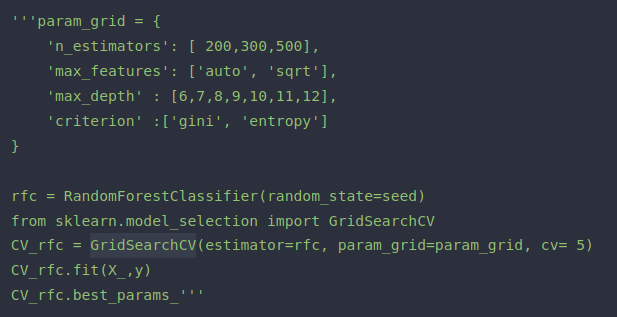
\includegraphics[width=0.8\textwidth]{imagenes/sub10-grid.png}
\caption{GridSearchCV(RFC) - sub10}
\end{figure}


Tras eso, realizo un ajuste de parámetros en base a lo obtenido.

\begin{figure}[H]
\centering
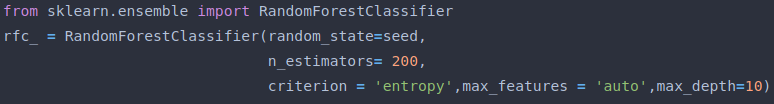
\includegraphics[width=0.8\textwidth]{imagenes/sub10-rfc.png}
\caption{RFC - sub10}
\end{figure}

\subsection{subida 11}

A partir de esta subida, comencé a crear un dataset de validación(parte pequeña de train como test). Haciendo fit de la parte de entrenamiento restante y predicción solo de la parte de test.

Para esta subida hice muchas pruebas variando \textit{estimators} y \textit{final\_estimator}. Dejando esta para la subida a kaggle.

\begin{figure}[H]
\centering
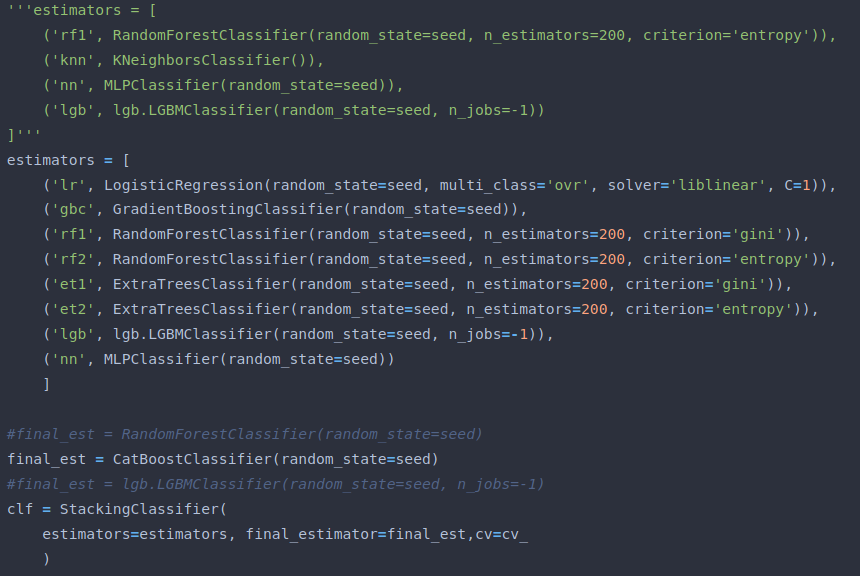
\includegraphics[width=0.8\textwidth]{imagenes/sub11.png}
\caption{StackingClassifier - sub11}
\end{figure}

\subsection{subida 14}

Usé como clasificador, CatBoostClassifier con los siguientes parámetros: $loss\_function='MultiClass'$, $eval\_metric='AUC'$.

\subsection{subida 15}

CatBoostClassifier con los siguientes parámetros: $loss\_function='MultiClass'$, $eval\_metric='Accuracy'$.

\subsection{subida 16}

Uso de SMOTETomek(combinando over y undersampling), con lgb como clasificador con tuning de parámetros. Viendo la baja accuracy que siempre tiene la clase 1, intento balancear algo las instancias de esa clase pasando de un 5.58\% a un 10.09\%. Siendo este realizado solo a la parte de entrenamiento de la parte de validación.

$clf=lgb.LGBMClassifier(random\_state=seed, n\_jobs=-1, colsample_bytree=0.5,num\_leaves=10, subsample=0.5)$

\begin{figure}[H]
\centering
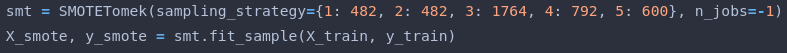
\includegraphics[width=0.8\textwidth]{imagenes/sub16-tomek.png}
\caption{SMOTETomek- sub16}
\end{figure}

\begin{figure}[H]

\begin{subfigure}{.5\textwidth}
  \centering
  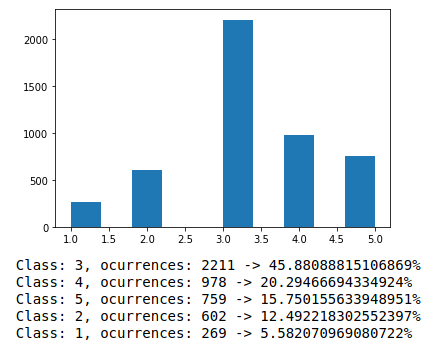
\includegraphics[width=0.8\textwidth]{imagenes/classes.png}
  \caption{Dataset original}
  \label{fig:sfig1}
\end{subfigure}%
\begin{subfigure}{.5\textwidth}
  \centering
  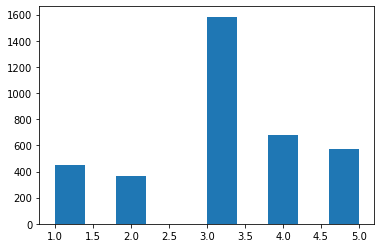
\includegraphics[width=0.8\textwidth]{imagenes/sub16-bal.png}
  \caption{Dataset tras SMOTETomek}
  \label{fig:sfig2}
\end{subfigure}

\caption{Aumento de instancias de la clase 1}
\label{fig:fig}
\end{figure}

\subsection{subida 17}

Igual que la anterior, pero en este caso \{1: 471, 2: 482, 3: 1764, 4: 792, 5: 600\} como diccionario y \textit{lgb} con configuración de parámetros por defecto.

\subsection{subida 18}

Igual que el anterior, pero intentando subir la precisión de la clase 1, $sample\_strategy=\{1: 600, 2: 602, 3: 2211, 4: 978, 5: 759\}$

\subsection{subida 20}

A la vista de no mejorar mucho el score, cambié las columnas usadas y la imputación de valores perdidos. Descarté el combustible porque no veía que pudiera ayudar a mejorar la precisión de las clases minoritarias y los asientos porque casi todos pertenecen a 5 asientos. Y añadí la marca del coche porque puede haber marcas destinadas a ciertos tipo de clientes.

Guardé en la columna \textit{Nombre}, solo la marca del coche dejando como 'mv' los valores perdidos. Al hacer el LabelEncoder, mediante la transformación inversa obtuve de nuevo los valores perdidos para imputarlos con \textit{KNNImputer}.
\section{Conclusiones}

Claramente se ha producido overfitting en muchos casos de intento de balanceo de clases y ajuste de parámetros, pero no conseguí que pudiera generalizar el modelo sin dejar de lado la precisión de este y así obtener mejores resultados en conjuntos de datos distintos a los de entrenamiento.

Durante y después de la realización de la práctica lo que más he notado es lo dificil que es llevar lo teórico a la parte práctica. Al final he obtenido el mejor resultado de un modelo configurado por defecto y un oversampling específico.

Debería haber probado más preprocesamientos así como un mejor estudio de las columnas a elegir. Quizás también más clasificadores, pero el ultimo que probé OneVersusOne, me seguía yendo peor en local así que pensé que podría estar limitandome el preprocesamiento de los datos y/o elección de las columnas.


%%%%%%%%%%%%%%%%%%%%%%%%%%%%% Referencias %%%%%%%%%%%%%%%%%%%%%%%%%%%%%
%\renewcommand{\refname}{\centering REFERENCIAS} %Centrar%
%\addcontentsline{toc}{section}{Referencias} % añade referencias al indice

\nocite{*}
\bibliographystyle{unsrt}
\bibliography{references}


\end{document}